\documentclass{../../../oss-classkick}

\begin{document}
\genheader

\gentitle{C}{ROTATIONAL MOTION}

\genmultidirections

\gengravity

\raggedcolumns
\begin{multicols*}{2}
  \begin{enumerate}[leftmargin=18pt]

%  \item Linear acceleration is to force as angular acceleration is to
%    \begin{enumerate}[noitemsep,topsep=0pt,leftmargin=18pt,label=(\Alph*)]
%    \item kinetic energy
%    \item angular velocity
%    \item rotational inertia
%    \item torque
%    \item angular momentum
%    \end{enumerate}
    
  \item A meter stick of mass \SI{.1}{\kilo\gram} rests on a table as shown. A
    length of \SI{40}{\centi\metre} extends over the edge of the table. How far
    from the edge of the table could a \SI{.05}{\kilo\gram} mass be placed on
    the meter stick so that the stick just begins to tip?
    \begin{center}
      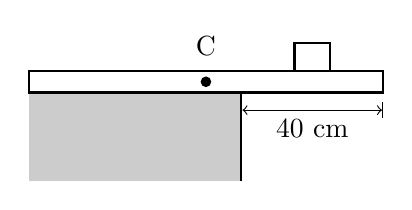
\begin{tikzpicture}[scale=4.5]
        \fill[gray!40](0,-.25) rectangle(.6,0);
        \begin{scope}[thick]
          \draw(0,0) rectangle(1,.06);
          \draw(.6,0)--(.6,-.25);
          \draw(.75,.06) rectangle (.85,.14);
        \end{scope}
        \draw[|<->|](.6,-.05)--(1,-.05) node[midway,below]{40 cm};
        \fill(.5,.03) circle(.015);
        \node at (.5,.13){C};
      \end{tikzpicture}
    \end{center}
    \begin{enumerate}[nosep,leftmargin=18pt,label=(\Alph*)]
    \item\SI{5}{\centi\metre}
    \item\SI{10}{\centi\metre}
    \item\SI{15}{\centi\metre}
    \item\SI{20}{\centi\metre}
    \item\SI{30}{\centi\metre}
    \end{enumerate}
    
%  \item A meter stick is balanced on a fulcrum at its center, as shown. A mass
%    of \SI{5}{\kilo\gram} is hung on the left end of the stick, and a mass of
%    \SI{2}{\kilo\gram} is hung on the right end. In order to balance the
%    system, a mass $m$ is hung at the 25-cm mark on the right
%    side. What is the value of the mass $m$?
%    \begin{center}
%      \pic{.33}{beam2.png}
%    \end{center}
%    \begin{enumerate}[noitemsep,topsep=0pt,leftmargin=18pt,label=(\Alph*)]
%    \item\SI{12}{\kilo\gram}
%    \item\SI{6 }{\kilo\gram}
%    \item\SI{4 }{\kilo\gram}
%    \item\SI{3 }{\kilo\gram}
%    \item\SI{2 }{\kilo\gram}
%    \end{enumerate}
    
  \item A metal bar of constant density and weight $W$ is attached to a pivot on
    the wall at point $P$ and supported by a rope that makes an angle of
    \ang{60} with the vertical wall. The reaction force exerted by the pivot on
    the bar at point P is best represented by which arrow?
    \begin{center}
      \pic{.25}{metal-bar.png}
    \end{center}
    \begin{enumerate}[itemsep=4.5pt,topsep=0pt,leftmargin=18pt,label=(\Alph*)]
    \item{\Large $\nearrow$}
    \item{\Large $\uparrow$}
    \item{\Large $\downarrow$}
    \item{\Large $\nwarrow$}
    \item{\Large $\searrow$}
    \end{enumerate}


  \item A ballet dancer is spinning around a vertical axis with her arms fully
    extended. How are her angular momentum and kinetic energy affected
    as she pulls her arms in toward her body as she spins?
    \begin{enumerate}[noitemsep,topsep=0pt,leftmargin=18pt,label=(\Alph*)]
    \item Her angular momentum remains constant, but her kinetic energy
      increases.
    \item Her angular momentum increases, but her kinetic energy remains
      constant.
    \item Her angular momentum decreases, but her kinetic energy remains
      constant.
    \item Her angular momentum increases, but her kinetic energy decreases.
    \item Both her angular momentum and kinetic energy remain constant.
    \end{enumerate}
    \vspace{.7in}
    
  \item A particle of mass $m$ moves with a constant speed $v$ at a distance
    $x_0$ parallel to the $y$-axis as shown. When the particle is in the
    position shown below, the magnitude of its angular momentum relative to the
    origin is
    \begin{center}
      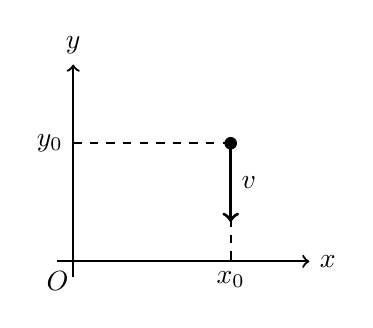
\begin{tikzpicture}
        \fill(2,1.5) circle(.08);
        \begin{scope}[thick]
          \draw[->](-.2,0)--(3,0) node[right]{$x$} node[pos=0,below]{$O$};
          \draw[->](0,-.2)--(0,2.5) node[above]{$y$};
          \draw[dashed](0,1.5)--(2,1.5) node[pos=0,left]{$y_0$}
          --(2,0)node[below]{$x_0$};
        \end{scope}
        \draw[very thick,->](2,1.5)--(2,.5) node[midway,right]{$v$};
      \end{tikzpicture}
    \end{center}
    \begin{enumerate}[itemsep=4pt,topsep=0pt,leftmargin=18pt,label=(\Alph*)]
    \item $mvx_0$
    \item $mvy_0$
    \item $mv\sqrt{x_0^2+y_0^2}$
    \item $\displaystyle\frac{mv}{\sqrt{x_0^2+y_0^2}}$
    \item zero
    \end{enumerate}
    \columnbreak
    
  \item A uniform rod of length $L$ and mass $m$ has a rotational inertia of
    $\displaystyle \frac1{12}mL^2$ about its center. A particle, also of mass
    $m$, is attached to one end of the stick. The combined rotational inertia of
    the stick and particle about the center of the rod is
     \begin{center}
      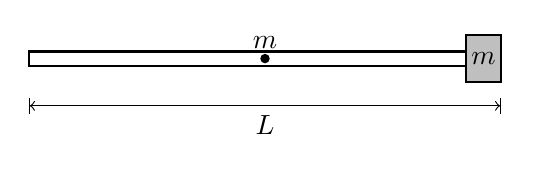
\begin{tikzpicture}[scale=3]
        \draw[thick](-1,-.03) rectangle (1,.03);
        \fill(0,0) circle(.02) node[above]{$m$};
        \draw[thick,fill=gray!50](.85,-.1) rectangle(1,.1) node[midway]{$m$};
        \draw[|<->|](-1,-.2)--(1,-.2) node[midway,below]{$L$};
      \end{tikzpicture}
    \end{center}
    \begin{enumerate}[itemsep=4pt,topsep=0pt,leftmargin=18pt,label=(\Alph*)]
    \item$\displaystyle\frac{mL^2}{3}$
    \item$\displaystyle\frac{12mL^2}{13}$
    \item$\displaystyle\frac{13mL^2}{12}$
    \item$\displaystyle\frac{mL^2}{156}$
    \item$\displaystyle\frac{13mL^2}{156}$
    \end{enumerate}

  \item A hoop of radius $R$ and mass $m$ has a rotational inertia of $mR^2$.
    The hoop rolls without slipping along a horizontal floor with a constant
    speed $v$ and then rolls up a long incline. The hoop can roll up the
    incline to a maximum vertical height of
    \begin{center}
      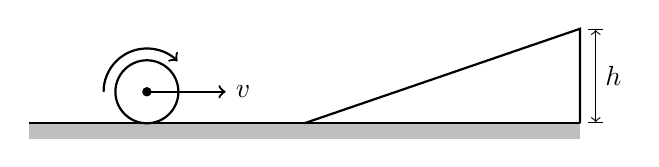
\begin{tikzpicture}
        \fill[gray!50](0,-.2) rectangle(7,0);
        \begin{scope}[thick]
          \draw(0,0)--(7,0);
          \draw(3.5,0)--(7,1.2)--(7,0);
          \draw(1.5,.4) circle(.4);
          \fill(1.5,.4) circle(.06);
          \draw[->](1.5,.4)--(2.5,.4) node[right]{$v$};
          \draw[->](.95,.4) arc(180:45:.55);
        \end{scope}
        \draw[|<->|](7.2,0)--(7.2,1.2) node[midway,right]{$h$};
      \end{tikzpicture}
    \end{center}
    \begin{enumerate}[nosep,leftmargin=18pt,label=(\Alph*)]
    \item$\displaystyle\frac{v^2}{g}$
    \item$\displaystyle\frac{2v^2}{g}$
    \item$\displaystyle\frac{v^2}{2g}$
    \item$\displaystyle\frac{4v^2}{g}$
    \item$\displaystyle\frac{v^2}{4g}$
    \end{enumerate}
    
  \item Two disks are fixed to a vertical axle that is rotating with a constant
    angular speed $\omega$. The smaller disk has a mass $m$ and a radius $r$,
    and the larger disk has a mass $2m$ and radius $2r$. The general equation
    for the rotational inertia of a disk of mass $M$ and radius $R$ is
    $\frac12MR^2$. The ratio of the angular momentum of the larger disk to
    the smaller disk is
    \begin{center}
      \pic{.25}{2disks.png}
    \end{center}
    \begin{enumerate}[noitemsep,topsep=0pt,leftmargin=18pt,label=(\Alph*)]
    \item$1:4$
    \item$4:1$
    \item$1:2$
    \item$2:1$
    \item$8:1$
    \end{enumerate}
    \columnbreak
    
  \item A light rod has a mass attached at each end. At one end is a
    \SI{6}{\kilo\gram} mass, and at the other end is a \SI{3}{\kilo\gram} mass.
    An axis can be placed at any of the points shown. Through which point
    should an axis be placed so that the rotational inertia is the greatest
    about that axis?
     \begin{center}
      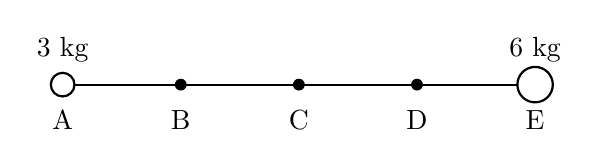
\begin{tikzpicture}[scale=1.5]
        \begin{scope}[thick]
          \draw(0,0) circle(.1);
          \draw(4,0) circle(.15);
          \draw(.1,0)--(3.85,0);
        \end{scope}
        \fill (1,0) circle(.05);
        \fill (2,0) circle(.05);
        \fill (3,0) circle(.05);
        \node at (0,-.3){A};
        \node at (1,-.3){B};
        \node at (2,-.3){C};
        \node at (3,-.3){D};
        \node at (4,-.3){E};
        \node at (0,.3){3 kg};
        \node at (4,.3){6 kg};
      \end{tikzpicture}
    \end{center}
    \begin{enumerate}[nosep,leftmargin=18pt,label=(\Alph*)]
    \item A
    \item B
    \item C
    \item D
    \item E
    \end{enumerate}

  \item A light rod of negligible mass is pivoted at point $P$ a distance $L$
    from one end as shown. A mass $m$ is attached to the left end of the rod at
    a distance of $3L$ from the pivot, and another mass $4m$ is attached to the
    other end a distance $L$ from the pivot. The system begins from rest in the
    horizontal position. The net torque acting on the system due to
    gravitational forces is
    \begin{center}
      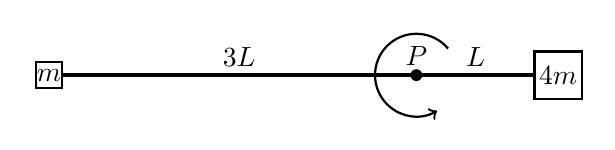
\begin{tikzpicture}[scale=1.5]
        \draw[very thick](-3,0)--(1,0);
        \draw[thick](1,-.2) rectangle(1.4,.2) node[midway]{$4m$};
        \draw[thick](-3,-.11) rectangle(-3.22,.11) node[midway]{$m$};
        \fill(0,0) circle(.05) node[above]{$P$};
        \node at (.5,.15){$L$};
        \node at (-1.5,.15){$3L$};
        \draw[thick,->,rotate=40](.35,0) arc(0:260:.35);
      \end{tikzpicture}
    \end{center}
    \begin{enumerate}[nosep,leftmargin=18pt,label=(\Alph*)]
    \item $4mgL$ clockwise
    \item $3mgL$ clockwise
    \item $3mgL$ counterclockwise
    \item $mgL$ counterclockwise
    \item $mgL$ clockwise
    \end{enumerate}
    \vspace{.7in}
    
  \item The angular acceleration of the system when it is released from rest is
    \begin{enumerate}[itemsep=4pt,topsep=0pt,leftmargin=18pt,label=(\Alph*)]
    \item zero
    \item $\displaystyle\frac{g}{5L}$
    \item $\displaystyle\frac{g}{4L}$
    \item $\displaystyle\frac{g}{13L}$
    \item $\displaystyle\frac{g}L$
    \end{enumerate}

  \item Two wheels are attached to each other and fixed so that they can only
    turn together. The smaller wheel has a radius of $r$ and the larger wheel
    has a radius of $3r$. The two wheels can rotate together on a frictionless
    axle. Three forces act tangentially on the edge of the wheels as shown.
    The magnitude of the net torque acting on the system of wheels is
    \begin{center}
      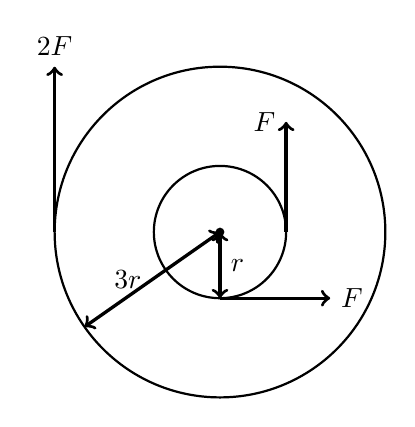
\begin{tikzpicture}[scale=.7]
        \begin{scope}[thick]
          \draw(0,0) circle(1.2);
          \draw(0,0) circle(3);
          \fill(0,0) circle(.08);
        \end{scope}
        \begin{scope}[very thick]
          \draw[<->](0,0)--(0,-1.2) node[midway,right]{$r$};
          \draw[<->,rotate=-55](0,0)--(0,-3) node[midway,left]{$3r$};
          \draw[->](0,-1.2)--(2,-1.2) node[right]{$\mb{F}$};
          \draw[->](1.2,0)--(1.2,2) node[left]{$\mb{F}$};
          \draw[->](-3,0)--(-3,3) node[above]{$2\mb{F}$};
        \end{scope}
      \end{tikzpicture}
    \end{center}
    \begin{enumerate}[nosep,leftmargin=18pt,label=(\Alph*)]
    \item$Fr$
    \item$2Fr$
    \item$3Fr$
    \item$4Fr$
    \item$6Fr$
    \end{enumerate}
    \columnbreak
    
  \item A disk is mounted on a fixed axle. The rotational inertia of the disk is
    $I$. The angular velocity of the disk is decreased from $\omega_i$ to
    $\omega_f$ during a time $\Delta t$ due to friction in the axle. The
    magnitude of the average net torque acting on the wheel is
    \begin{enumerate}[noitemsep,topsep=0pt,leftmargin=18pt,label=(\Alph*)]
    \item $\displaystyle\frac{\omega_f-\omega_i}{\Delta t}$
    \item $\displaystyle\frac{(\omega_f-\omega_i)^2}{\Delta t}$
    \item $\displaystyle\frac{I(\omega_f-\omega_i)}{\Delta t}$
    \item $\displaystyle\frac{I(\omega_f-\omega_i)^2}{\Delta t}$
    \item $\displaystyle\frac{I(\omega_f-\omega_i)}{\Delta t^2}$
    \end{enumerate}
    
  \item The average power developed by the friction in the axle of the disk
    from the previous question to bring it to a complete stop is
    \begin{enumerate}[itemsep=4pt,topsep=0pt,leftmargin=18pt,label=(\Alph*)]
    \item $\displaystyle\frac{\omega_i}{\Delta t}$
    \item $\displaystyle\frac{(\omega_i)^2}{\Delta t}$
    \item $\displaystyle\frac{I\omega_i}{2\Delta t}$
    \item $\displaystyle\frac{I\omega_i^2}{2\Delta t}$
    \item $\displaystyle\frac{I\omega_i}{\Delta t^2}$
    \end{enumerate}    

  \item Astronauts are conducting an experiment in a negligible gravity
    environment. Two spheres of mass $m$ are attached to either end of a light
    rod. As the rod and spheres float motionless in space, an astronaut
    launches a piece of sticky clay, also of mass $m$, toward one of the spheres
    so that the clay strikes and sticks to the sphere perpendicular to the rod.
    Which of the following statements is true of the motion of the rod, clay,
    and spheres after the collision?
    \begin{center}
      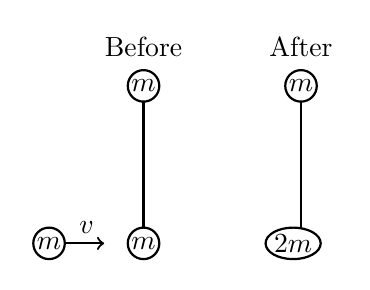
\begin{tikzpicture}
        \begin{scope}[thick]
          \draw(0,0) circle(.2) node{$m$};
          \draw(0,2) circle(.2) node{$m$};
          \draw(0,.2)--(0,1.8);
          \draw(-1.2,0) circle(.2) node{$m$};
          \draw[->](-1,0)--(-.5,0) node[above left]{$v$};

          \draw(1.9,0) ellipse(.35 and .2) node{$2m$};
          \draw(2,2) circle(.2) node{$m$};
          \draw(2,.2)--(2,1.8);
        \end{scope}
        \node at (0,2.5) {Before};
        \node at (2,2.5) {After};
      \end{tikzpicture}
    \end{center}
    \begin{enumerate}[nosep,leftmargin=18pt,label=(\Alph*)]
    \item Linear momentum is not conserved, but angular momentum is conserved.
    \item Angular momentum is not conserved, but linear momentum is conserved.
    \item Kinetic energy is conserved, but angular momentum is not conserved.
    \item Kinetic energy is conserved, but linear momentum is not conserved.
    \item Both linear momentum and angular momentum are conserved, but kinetic
      energy is not conserved.
    \end{enumerate}
    \vspace{.7in}
    
  \item A rod of mass $M$, length $L$, and rotational inertia $I$ hangs at rest
    from a frictionless axle as shown. A ball of mass $m$ with a speed $v$
    strikes therod perpendicularly at the end of the rod. As a result of the
    collision, the ball stops. The angular speed of the rod immediately after
    the collision is
    \begin{center}
      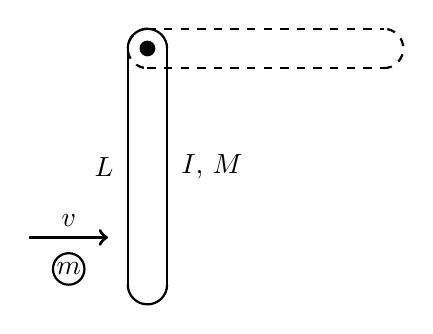
\begin{tikzpicture}
        \fill(0,0) circle(.1);
        \begin{scope}[thick]
          \draw(.25,0) arc(0:180:.25);
          \draw(-.25,0)--(-.25,-3);
          \draw( .25,0)--( .25,-3);
          \draw(-.25,-3) arc(180:360:.25);
          \begin{scope}[dashed,rotate=90]
            \draw(.25,0) arc(0:180:.25);
            \draw(-.25,0)--(-.25,-3);
            \draw( .25,0)--( .25,-3);
            \draw(-.25,-3) arc(180:360:.25);
          \end{scope}
          \draw(-1,-2.8) circle(.2) node{$m$};
          \draw[very thick,->](-1.5,-2.4)--(-.5,-2.4) node[midway,above]{$v$};
          \node[left] at (-.3,-1.5) {$L$};
          \node[right] at (.3,-1.5) {$I$, $M$};
        \end{scope}
      \end{tikzpicture}
    \end{center}
    \begin{enumerate}[nosep,leftmargin=18pt,label=(\Alph*)]
    \item $vL$
    \item $\displaystyle\frac{v}L$
    \item $\displaystyle\frac{mv}I$
    \item $\displaystyle\frac{mvL}I$
    \item $\displaystyle\frac{mv}{IL}$
    \end{enumerate}
  \end{enumerate}
  \columnbreak

  \textbf{Questions \ref{hollow1}--\ref{hollow2}} A hollow sphere of mass $m$
  and radius $R$ begins from rest at a height $h$ and rolls down a rough
  inclined plane. The rotational inertia of the hollow sphere is
  $\displaystyle\frac23mR^2$.
  \begin{center}
    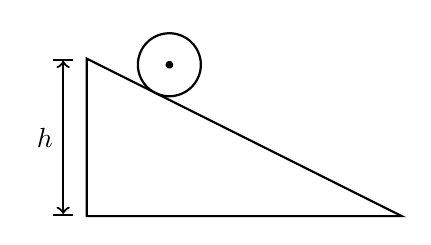
\begin{tikzpicture}
      \begin{scope}[thick]
        \draw(0,0)--(-4,0)--(-4,2)--cycle;
        \draw[|<->|](-4.3,2)--(-4.3,0) node[midway,left]{$h$};
      \end{scope}
      \begin{scope}[thick,rotate=-atan(2/4)]
        \draw(-3.5,.4) circle(.4);
        \fill(-3.5,.4) circle(.05);
      \end{scope}
    \end{tikzpicture}
  \end{center}
  \begin{enumerate}[leftmargin=18pt,resume]
  \item  Which of the following diagrams best represents the forces acting on
    the sphere as it rolls down the plane?
    \begin{enumerate}[nosep,leftmargin=18pt,label=(\Alph*)]
    \item 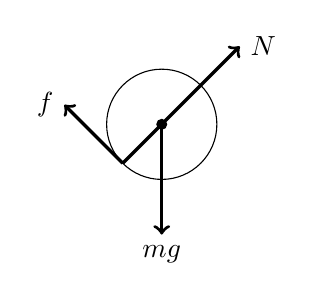
\begin{tikzpicture}[scale=.7]
      \draw(0,0) circle(1);
      \fill(0,0) circle(.1);
      \begin{scope}[very thick,->]
        \draw (0,0)--(0,-2) node[below]{$mg$};
        \draw[rotate=45](-1,0)--(2,0) node[right]{$N$};
        \draw[rotate=45](-1,0)--(-1,1.5) node[left]{$f$};
      \end{scope}
    \end{tikzpicture}

    \item 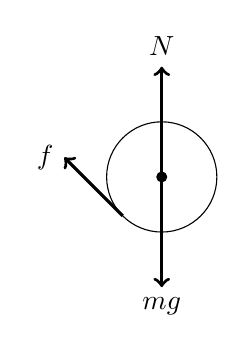
\begin{tikzpicture}[scale=.7]
      \draw(0,0) circle(1);
      \fill(0,0) circle(.1);
      \begin{scope}[very thick,->]
        \draw (0,0)--(0,-2) node[below]{$mg$};
        \draw (0,0)--(0,2) node[above]{$N$};
        \draw[rotate=45](-1,0)--(-1,1.5) node[left]{$f$};
      \end{scope}
    \end{tikzpicture}

    \item 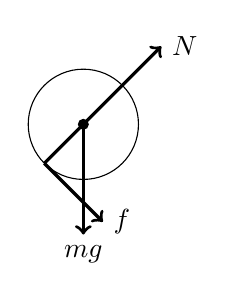
\begin{tikzpicture}[scale=.7]
      \draw(0,0) circle(1);
      \fill(0,0) circle(.1);
      \begin{scope}[very thick,->]
        \draw (0,0)--(0,-2) node[below]{$mg$};
        \draw[rotate=45](-1,0)--(2,0) node[right]{$N$};
        \draw[rotate=45](-1,0)--(-1,-1.5) node[right]{$f$};
      \end{scope}
    \end{tikzpicture}

    \item 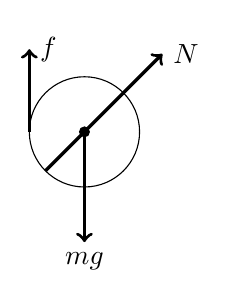
\begin{tikzpicture}[scale=.7]
      \draw(0,0) circle(1);
      \fill(0,0) circle(.1);
      \begin{scope}[very thick,->]
        \draw (0,0)--(0,-2) node[below]{$mg$};
        \draw[rotate=45](-1,0)--(2,0) node[right]{$N$};
        \draw(-1,0)--(-1,1.5) node[right]{$f$};
      \end{scope}
    \end{tikzpicture}
      
    \item 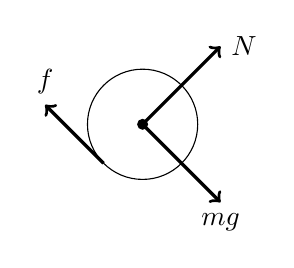
\begin{tikzpicture}[scale=.7]
      \draw(0,0) circle(1);
      \fill(0,0) circle(.1);
      \begin{scope}[very thick,->]
        \draw[rotate=45](0,0)--(0,-2) node[below]{$mg$};
        \draw[rotate=45](0,0)--(2,0) node[right]{$N$};
        \draw[rotate=45](-1,0)--(-1,1.5) node[above]{$f$};
      \end{scope}
    \end{tikzpicture}
    \end{enumerate}
    \label{hollow1}
    
  \item The speed of the sphere when it reaches the bottom of the plane is
    \begin{enumerate}[nosep,leftmargin=18pt,label=(\Alph*)]
    \item$\displaystyle\frac{8gh}5$
    \item$\displaystyle\frac{6gh}5$
    \item$\displaystyle\frac{5gh}6$
    \item$\displaystyle\frac{7gh}{10}$
    \item$\displaystyle\frac{gh}2$
    \end{enumerate}
    \label{hollow2}
    \columnbreak
    
  \item One end of a stick of length $L$, rotational inertia $I$, and mass $m$
    is pivoted on an axle with negligible friction at point $P$. The other end
    is tied to a string and held in a horizontal position. When the string is
    cut, the stick rotates counterclockwise. The angular speed $\omega$ of the
    stick when it reaches the bottom of its swing is
    \cpic{.32}{end-of-stick}
    \begin{enumerate}[nosep,leftmargin=18pt,label=(\Alph*)]
    \item$\displaystyle\frac{mgL}I$
    \item$\displaystyle\sqrt{\frac{mgL}I}$
    \item$\displaystyle\sqrt{\frac{2mgL}I}$
    \item$\displaystyle\sqrt{\frac{mgL}{2I}}$
    \item$\displaystyle\sqrt{\frac{4mgL}I}$
    \end{enumerate}
  \end{enumerate}
\end{multicols*}
\newpage

\genfreetitle{C}{ROTATIONAL MOTION}{6}

\genfreedirections

% TAKEN FROM THE 2015 AP PHYSICS C FREE-RESPONSE QUESTION MECH 3
\begin{center}
  \pic{.4}{thinrod1}
\end{center}
\begin{enumerate}
\item A uniform, thin rod of length $L$ and mass $M$ is allowed to pivot about
  its end, as shown in the figure above.
  \begin{enumerate}[leftmargin=15pt]
  \item Using integral calculus, derive the rotational inertia for the rod
    around its end to show that it is $ML^2/3$.
  \end{enumerate}
  \begin{center}
    \pic{.4}{thinrod2}
  \end{center}
  The rod is fixed at one end and allowed to fall from the horizontal
  position $A$ through the vertical position $B$.
  \begin{enumerate}[leftmargin=15pt,resume]
  \item Derive an expression for the velocity of the free end of the rod at
    position $B$. Express your answer in terms of $M$, $L$, and physical
    constants, as appropriate.
  \end{enumerate}
  \newpage
  An experiment is designed to test the validity of the expression found in
  part (b). A student uses rods of various lengths that all have a uniform
  mass distribution. The student releases each of the rods from the horizontal
  position $A$ and uses photogates to measure the velocity of the free end at
  position $B$. The data are recorded below.
  \begin{center}
    \def\arraystretch{1.45}
    \begin{tabular}{|c|c|c|c|c|c|c|}
      \hline
      Length (m)     & 0.25 & 0.50 & 0.75 & 1.00 & 1.25 & 1.50\\\hline
      Velocity (m/s) & 2.7  & 3.8  & 4.6  & 5.2  & 5.8  & 6.3 \\\hline
      & & & & & & \\\hline
      & & & & & & \\\hline
    \end{tabular}
    \def\arraystretch{1}
  \end{center}

  \begin{enumerate}[resume]
  \item Indicate below which quantities should be graphed to yield a straight
    line whose slope could be used to calculate a numerical value for the
    acceleration due to gravity $g$.

    \vspace{.1in}Horizontal axis: \underline{\hspace{1in}}

    \vspace{.1in}Vertical axis: \underline{\hspace{1in}}

    \vspace{.1in}Use the remaining rows in the table above, as needed, to
    record any quantities that you indicated that are not given. Label each row
    you use and include units.

  \item Plot the straight line data points on the grid below. Clearly scale and
    label all axes, including units as appropriate. Draw a straight line that
    best represents the data.
    \begin{center}
      \pic{.9}{graph-paper}
    \end{center}
  \item
    \begin{enumerate}
    \item Using your straight line, determine an experimental value for $g$.
    \item Describe two ways in which the effects of air resistance could be
      reduced.
    \end{enumerate}
  \end{enumerate}
  \newpage

\item A uniform sphere of mass $M$ and radius $R$ is free to rotate, without
  friction, about a horizontal axis through its center. A string is wrapped
  around the sphere and is attached to a body of mass $m$ as shown in the
  figure below. Find
  \begin{center}
    \vspace{-.2in}
    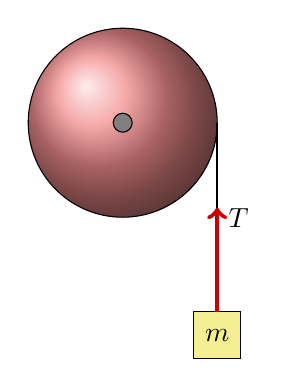
\begin{tikzpicture}[scale=.6]
      \tikzstyle{balloon}=[ball color=red!80!gray!50];
      \shade[balloon] (0,0) circle (2);% node[below right]{$m$};
      \draw(0,0) circle(2);
      \draw[fill=gray](0,0) circle(.2);
      \draw[thick](2,0)--(2,-4);
      \draw[fill=yellow!80!gray!50](1.5,-4) rectangle(2.5,-5)
      node[midway,black]{$m$};
      \draw[ultra thick,red!80!black,->](2,-4)--(2,-1.8)
      node[pos=.9,right,black]{$T$};
    \end{tikzpicture}
  \end{center}
  \begin{enumerate}
  \item the acceleration of the body, and
  \item the tension in the string.
  \end{enumerate}
  \newpage

\item A uniform cylinder of mass $M$ and radius $R$ has a string wrapped around
  it. The string is held fixed, and the cylinder falls vertically as shown in
  the figure below. Find
  \begin{center}
    \vspace{-.3in}
    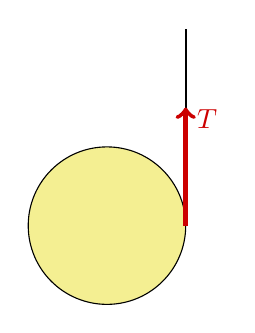
\begin{tikzpicture}[scale=.5]
      \draw[fill=yellow!80!gray!50](0,0) circle(2);
      \draw[thick](2,0)--(2,5);
      \draw[ultra thick,red!80!black,->](2,0)--(2,3) node[pos=.9,right]{$T$};
    \end{tikzpicture}
  \end{center}
  \begin{enumerate}
  \item the acceleration of the body, and
  \item the tension in the string.
  \end{enumerate}
  \newpage

  \begin{center}
    \pic{.65}{disc1}
    \end{center}

\item A large circular disk of mass $m$ and radius $R$ is initially stationary
  on a horizontal icy surface. A person of mass $m/2$ stands on the edge of the
  disk. Without slipping on the disk, the person throws a large stone of mass
  $m/20$ horizontally at initial speed $v_0$ from a height $h$ above the ice in
  a radial direction, as shown in the figures above. The coefficient of
  friction between the disk and the ice is $\mu$. All velocities are measured
  relative to the ground. The time it takes to throw the stone is negligible.
  Express all algebraic answers in terms of $m$, $R$, $v_0$, $h$, $m$, and
  fundamental constants, as appropriate.
  \begin{enumerate}
  \item Derive an expression for the length of time it will take the stone to
    strike the ice.
  \item Assuming that the disk is free to slide on the ice, derive an
    expression for the speed of the disk and person immediately after the stone
    is thrown.
  \item Derive an expression for the time it will take the disk to stop sliding.
  \end{enumerate}
  \begin{center}
    \pic{.25}{disc2}
  \end{center}
  The person now stands on a similar disk of mass $m$ and radius $R$ that has a
  fixed pole through its center so that it can only rotate on the ice. The
  person throws the same stone horizontally in a tangential direction at
  initial speed $u_0$, as shown in the figure above. The rotational inertia of
  the disk is $mR^2/2$.
  \begin{enumerate}[resume]
  \item Derive an expression for the angular speed $\omega$ of the disk
    immediately after the stone is thrown.
  \item The person now stands on the disk at rest $R/2$ from the center of the
    disk. The person now throws the stone horizontally with a speed $v_0$ in
    the same direction as in part (d). Is the angular speed of the disk
    immediately after throwing the stone from this new position greater than,
    less than, or equal to the angular speed found in part (d)?

    \vspace{.1in}
    \underline{\hspace{.3in}} Greater than\hspace{.2in}
    \underline{\hspace{.3in}} Less than\hspace{.2in}
    \underline{\hspace{.3in}} Equal to
    
    \vspace{.1in}Justify your answer.
  \end{enumerate}
  \newpage
  
\item A uniform ball of radius $r$ rolls without slipping along the
  loop-the-loop track in the figure below. The ball starts at rest at a height
  of $h$ above the bottom of the loop.
  \cpic{.55}{roll-ball}
  \begin{enumerate}
  \item If it is not to leave the track at the top of the loop, what is the
    least value $h$ can have (in terms of radius $R$ of the loop)?
  \item What would $h$ have to be if, instead of rolling, the ball slides
    without friction?
  \end{enumerate}
  \newpage
  
  \begin{center}
    \pic{.3}{rotating-disk}
  \end{center}
\item A disk of mass $M =\SI{2.}{\kilo\gram}$ and radius $R=\SI{.10}{\metre}$ is
  supported by a rope of negligible mass, as shown above. The rope is attached
  to the ceiling at one end and passes under the disk. The other end of the
  rope is pulled upward with a force $F_A$. The rotational inertia of the disk
  around its center is $MR^2/2$.
  \begin{enumerate}
  \item Calculate the magnitude of the force $F_A$ necessary to hold the disk
    at rest.
  \end{enumerate}
  At time $t=0$, the force $F_A$ is increased to 12 N, causing the disk to
  accelerate upward. The rope does not slip on the disk as the disk rotates.
  \begin{enumerate}[resume]
  \item Calculate the linear acceleration of the disk.
  \item Calculate the angular speed of the disk at $t=\SI{3.}{\second}$.
  \item Calculate the increase in total mechanical energy of the disk from
    $t=0$ to $t=\SI{3.}{\second}$.
  \item The disk is replaced by a hoop of the same mass and radius. Indicate
    whether the linear acceleration of the hoop is greater than, less than, or
    the same as the linear acceleration of the disk.

    \vspace{.1in}   
    \underline{\hspace{.3in}} Greater than\hspace{.2in}
    \underline{\hspace{.3in}} Less than\hspace{.2in}
    \underline{\hspace{.3in}} The same as

    \vspace{.1in}Justify your answer.
  \end{enumerate}
\end{enumerate}
\end{document}
